\subsection{Đề 2}
\Opensolutionfile{ans}[ans/ans-2-GK1-De2-LC]
\caulc
	\begin{ex}%[2D1H1-2]
	\immini{
		Cho hàm số $y=f(x)$ có đồ thị như Hình $1$. Hàm số $y=f(x)$ đồng biến trên khoảng
		\choice
		{\True $(5;+\infty)$}
		{$(3;5)$}
		{$(0;5)$}
		{$(3;+\infty)$}
	}{
		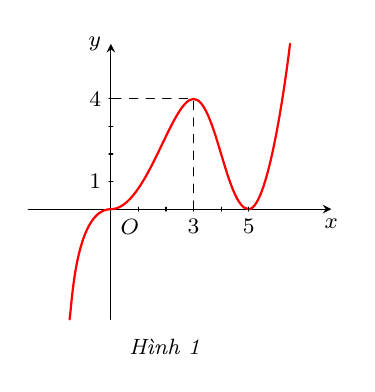
\begin{tikzpicture}[scale=0.7, font=\footnotesize, line join=round, line cap=round, >=stealth, xscale=0.5, yscale=0.5]
			\draw[->] (-3,0) -- (8,0) node[below] {$x$};
			\draw[->] (0,-4) -- (0,6) node[left] {$y$};
			\node at (0,0) [below right]{$O$};
			\coordinate (A) at (-1.5,-4);
			\coordinate (B) at (0,0);
			\coordinate (C) at (3,4);
			\coordinate (D) at (5,0);
			\coordinate (E) at (6.5,6);
			\draw[thick,red]
			(A) .. controls +(80:0.5) and +(180:1.3) ..
			(B) .. controls +(0:1.3) and +(180:.8) ..
			(C) .. controls +(0:.8) and +(180:.8) ..
			(D) .. controls +(0:.8) and +(180:0) .. (E);
			\foreach \x in {1,2,3,4,5}
			\draw[shift={(\x,0)},color=black] (0pt,2pt) -- (0pt,-2pt);
			\foreach \y in {1,2,3,4}
			\draw[shift={(0,\y)},color=black] (2pt,0pt) -- (-2pt,0pt);
			\draw[dashed] (3,0)node[below] {$3$}--(3,4)--(0,4)node[left] {$4$};
			\node at (5,0) [below]{$5$};
			\node at (0,1) [left]{$1$};
			\node at (2,-5){\text{\textit{Hình 1}}};
		\end{tikzpicture}
	}
	\loigiai{
		Từ hình vẽ, ta thấy hàm số $y=f(x)$ đồng biến trên khoảng $(-\infty;3)$ và $(5;+\infty)$.\\
		Từ các phương án, ta chọn hàm số $y=f(x)$ đồng biến trên khoảng $(5;+\infty)$.
	}
\end{ex}
%%%=============EX_2=============%%%
\begin{ex}%[2D1H2-2]
	\immini{
		Cho hàm số $y=f(x)$ có đồ thị như Hình $1$. Hàm số đạt cực đại tại
		\choice
		{$x=0$}
		{\True $x=3$}
		{$x=4$}
		{$x=5$}
	}{
		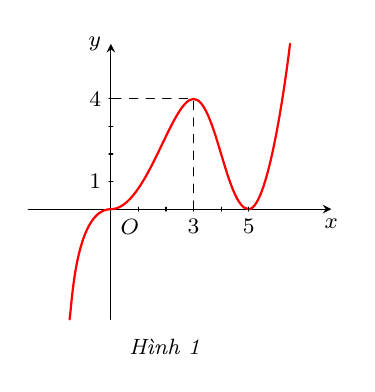
\begin{tikzpicture}[scale=0.7, font=\footnotesize, line join=round, line cap=round, >=stealth, xscale=0.5, yscale=0.5]
			\draw[->] (-3,0) -- (8,0) node[below] {$x$};
			\draw[->] (0,-4) -- (0,6) node[left] {$y$};
			\node at (0,0) [below right]{$O$};
			\coordinate (A) at (-1.5,-4);
			\coordinate (B) at (0,0);
			\coordinate (C) at (3,4);
			\coordinate (D) at (5,0);
			\coordinate (E) at (6.5,6);
			\draw[thick,red]
			(A) .. controls +(80:0.5) and +(180:1.3) ..
			(B) .. controls +(0:1.3) and +(180:.8) ..
			(C) .. controls +(0:.8) and +(180:.8) ..
			(D) .. controls +(0:.8) and +(180:0) .. (E);
			\foreach \x in {1,2,3,4,5}
			\draw[shift={(\x,0)},color=black] (0pt,2pt) -- (0pt,-2pt);
			\foreach \y in {1,2,3,4}
			\draw[shift={(0,\y)},color=black] (2pt,0pt) -- (-2pt,0pt);
			\draw[dashed] (3,0)node[below] {$3$}--(3,4)--(0,4)node[left] {$4$};
			\node at (5,0) [below]{$5$};
			\node at (0,1) [left]{$1$};
			\node at (2,-5){\text{\textit{Hình 1}}};
		\end{tikzpicture}
	}
	\loigiai{
		Từ hình vẽ, ta thấy hàm số $y=f(x)$ đạt cực đại tại $x=3$, $y_{\text{CĐ}}=4$.
	}
\end{ex}
%%%=============EX_3=============%%%
\begin{ex}%[2D1H2-1]
	Cho hàm số $y=\dfrac{x^2-4x+1}{x-4}$. Trong các khẳng định sau, khẳng định nào đúng?
	\choice
	{Hàm số đạt cực tiểu tại $x=3$, giá trị cực tiểu là $y=2$}
	{\True Hàm số đạt cực tiểu tại $x=5$, giá trị cực tiểu là $y=6$}
	{Hàm số đạt cực tiểu tại $x=3$, giá trị cực tiểu là $y=6$}
	{Hàm số đạt cực tiểu tại $x=5$, giá trị cực tiểu là $y=2$}
	\loigiai{
		Tập xác định $\mathscr{D}=\mathbb{R}\setminus \{4\}$.\\
		Ta có $y=x+\dfrac{1}{x-4} \Rightarrow y'=1-\dfrac{1}{(x-4)^2}=\dfrac{x^2-8x+15}{(x-4)^2}$;\\
		$y'=0 \Leftrightarrow x^2-8x+15=0 \Leftrightarrow \hoac{& x=3\\& x=5.}$\\
		Bảng biến thiên
		\begin{center}
			
\begin{tikzpicture}
				\tkzTabInit[nocadre=true,lgt=1.2,espcl=2.5,deltacl=0.6]
				{$x$ /0.6,$y'$ /0.6,$y$ /2}
				{$-\infty$,$3$,$4$,$5$,$+\infty$}
				\tkzTabLine{,+,$0$,-,d,-,$0$,+,}
				\tkzTabVar{-/$-\infty$,+/$2$,-D+/$-\infty$/$+\infty$,-/$6$,+/$+\infty$}
			\end{tikzpicture}
		\end{center}
		Vậy hàm số đạt cực tiểu tại $x=5$, giá trị cực tiểu là $y=6$.	
	}
\end{ex}
%%%=============EX_4=============%%%
\begin{ex}%[2D1H1-2]
	\immini{
		Đạo hàm của hàm số $y=f(x)$ là hàm số có đồ thị được cho trong Hình $2$. Hàm số $y=f(x)$ nghịch biến trên khoảng
		\choice
		{$(-1;3)$}
		{$(-3;1)$}
		{\True $(1;5)$}
		{$(3;+\infty)$}
	}{
		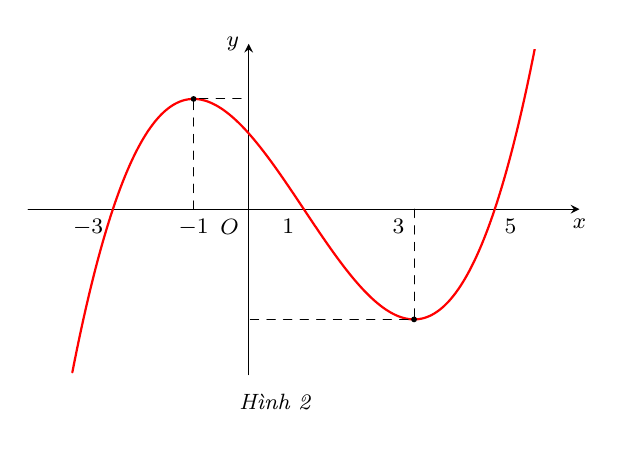
\begin{tikzpicture}[scale=0.7, font=\footnotesize, line join=round, line cap=round, >=stealth]
			\def\a{1} \def\b{-3} \def\c{-9} \def\d{11} % Hệ số
			\def\xt{-4} \def\xp{6} \def\yt{3} \def\yd{-3} % x_trái, x_phải, y_trên, y_dưới (giới hạn)
			\draw[->] (\xt,0)--(\xp,0) node [below]{$x$};
			\draw[->] (0,\yd)--(0,\yt) node [left]{$y$};
			\node at (0,0) [below left]{$O$};
			\clip (\xt+0.1,\yd-1) rectangle (\xp-0.1,\yt-0.1);
			\draw[thick,smooth,samples=300,domain=-3.2:\xp,red] plot(\x,{1/8*(\a*(\x)^3+\b*(\x)^2+\c*(\x)+\d)});
			\node at (-2.4641,0) [below left]{$-3$};
			\node at (1,0) [below left]{$1$};
			\draw[dashed] (-1,0) node [below]{$-1$}--(-1,2)--(0,2) (3,0) node [below left]{$3$}--(3,-2)--(0,-2);
			\node at (4.4641,0) [below right]{$5$};
			\fill (-1,2) circle (1.5pt) (3,-2) circle (1.5pt);
			\node at (0.5,-3.5){\text{\textit{Hình 2}}};
		\end{tikzpicture}
	}
	\loigiai{
		Từ đồ thị ta thấy $f'(x)<0 \Leftrightarrow x\in (-\infty;-3)\cup (1;5)$.\\
		Suy ra hàm số nghịch biến trên các khoảng $(-\infty;-3)$ và $(1;5)$.\\
		Từ các phương án, ta chọn hàm số nghịch biến trên khoảng $(1;5)$.
	}
\end{ex}
%%%=============EX_5=============%%%
\begin{ex}%[2D1H3-1]
	Giá trị nhỏ nhất của hàm số $y=\sqrt{x^2+2x+3}$ trên đoạn $[-2;3]$ là
	\choice
	{$\sqrt{3}$}
	{$\sqrt{30}$}
	{\True $\sqrt{2}$}
	{$0$}
	\loigiai{
		Xét hàm số $y=\sqrt{x^2+2x+3}=\sqrt{(x+1)^2+2}$.\\
		Tập xác định $\mathscr{D}=\mathbb{R}$.\\
		Ta có $y\geq\sqrt{2}$ với mọi $x\in [-2;3]$.\\
		Mặt khác $g(-1)=\sqrt{2}$, suy ra $\min\limits_{x\in [-2;3]} y=\sqrt{2}$.
	}
\end{ex}
%%%=============EX_6=============%%%
\begin{ex}%[2D1H4-1]
	Tiệm cận xiên của đồ thị hàm số $y=\dfrac{2x^3+3x^2-3}{x^2-1}$ là đường thẳng có phương trình
	\choice
	{\True $y=2x+3$}
	{$y=2x+1$}
	{$y=x+3$}
	{$y=x+1$}
	\loigiai{
		Xét hàm số $y=f(x)=\dfrac{2x^3+3x^2-3}{x^2-1}=2x+3+\dfrac{2x}{x^2-1}$.\\
		Tập xác định $\mathscr{D}=\mathbb{R}\setminus \{\pm 1\}$.\\
		Ta có $\lim\limits_{x\to -\infty} \left[f(x)-(2x+3)\right]=\lim\limits_{x\to -\infty} \dfrac{2x}{x^2-1}=0$ và $\lim\limits_{x\to +\infty} \left[f(x)-(2x+3)\right]=\lim\limits_{x\to +\infty} \dfrac{2x}{x^2-1}=0$.\\
		Do đó, đồ thị hàm số có tiệm cận xiên là đường thẳng $y=2x+3$.
	}
\end{ex}
%%%=============EX_7=============%%%
\begin{ex}%[2D1H4-1]
	Tiệm cận đứng của đồ thị hàm số $y=\dfrac{-2x+3}{5x+1}$ là đường thẳng có phương trình
	\choice
	{$y=-\dfrac{1}{5}$}
	{\True $x=-\dfrac{1}{5}$}
	{$y=-\dfrac{2}{5}$}
	{$x=-\dfrac{2}{5}$}
	\loigiai{
		Tập xác định $\mathscr{D}=\mathbb{R}\setminus \left\lbrace -\dfrac{1}{5}\right\rbrace$.\\
		Ta có $\lim\limits_{x\to \left(-\tfrac{1}{5}\right)^{-}} \dfrac{-2x+3}{5x+1}=-\infty$; và $\lim\limits_{x\to \left(-\tfrac{1}{5}\right)^{+}} \dfrac{-2x+3}{5x+1}=+\infty$.\\
		Suy ra $x=-\dfrac{1}{5}$ là một tiệm cận đứng của đồ thị hàm số đã cho.
	}
\end{ex}
%%%=============EX_8=============%%%
\begin{ex}%[2D1H1-1]
	Cho hàm số $y=\dfrac{-2x-3}{4-x}$. Trong các khẳng định sau, khẳng định nào đúng?
	\choice
	{Hàm số đồng biến trên $(-\infty;-4)$ và nghịch biến trên $(-4;+\infty)$}
	{Hàm số đồng biến trên $(-\infty;4)$ và $(4;+\infty)$}
	{\True Hàm số nghịch biến trên $(-\infty;4)$ và $(4;+\infty)$}
	{Hàm số nghịch biến trên $(-\infty;-4)$ và $(-4;+\infty)$}
	\loigiai{
		Tập xác định $\mathscr{D}=\mathbb{R}\setminus \{4\}$.\\
		Ta có $y=\dfrac{-2x-3}{-x+4} \Rightarrow y'=-\dfrac{11}{(4-x)^2}<0$, $\forall x\in \mathscr{D}$.\\
		Vậy hàm số nghịch biến trên $(-\infty;4)$ và $(4;+\infty)$.
	}
\end{ex}	
\begin{ex}%[2D1H1-1]
	\immini[thm]{ 
		Cho hàm số $y=f(x)$ có đạo hàm trên $\mathbb{R}$ và hàm số $y=f^\prime (x)$ có đồ thị như {\it Hình 31}.\\
		Hàm số $y=f(x)$ đồng biến trên khoảng:
		\choice[2]
		{$\left(-\infty;1\right)$}
		{\True $\left(0;1\right)$}
		{$\left(0;2\right)$}
		{$\left(1;2\right)$}
	}{
		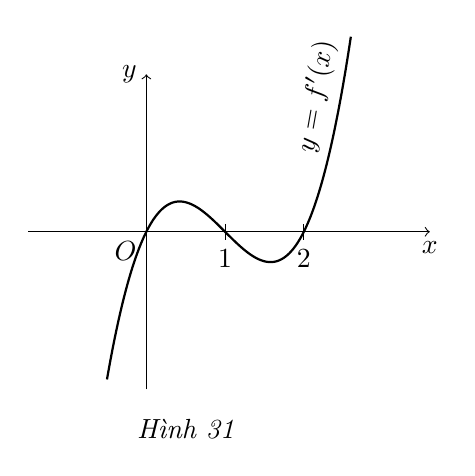
\begin{tikzpicture}
			
			\def\a{1}
			\def\b{-3}
			\def\c{2}
			\def\d{0}
			\def\f(#1){\a*((#1)^3)+\b*((#1)^2)+\c*(#1)+\d}
			\def\xmin{-.5}
			\def\xmax{2.6}
			\def\ymin{-1}
			\def\ymax{1}
			\draw[->] (\xmin-1,0)--(\xmax+1,0) node[below] { $x$};
			\draw[->] (0,\ymin-1)--(0,\ymax+1) node[left] { $y$};
			\draw (0,0) node [below left] { $O$};
			\foreach \x in {1,2}\draw (\x,0.1)--(\x,-0.1) node [below] { $\x$};
			%	\foreach \y in {-3,-2,-1,1,2,3}\draw (0.1,\y)--(-0.1,\y) node [left] { $\y$};
			%	\clip (\xmin,\ymin) rectangle (\xmax,\ymax);
			\draw[thick,smooth,samples=200] plot[domain=\xmin:\xmax] (\x,{\f(\x)});
			\draw (\xmax,{\f(\xmax)}) node [above left,rotate=80]{$y=f^\prime (x)$};	
			\node at (0.5,-2.5) {\it Hình 31};
			
		\end{tikzpicture}
	}
	
	\loigiai{
		Ta thấy đồ thị hàm số $y=f^\prime (x)$  phía trên trục $Ox$ trên  khoảng $\left(0;1\right)$ và $\left(2;+\infty\right)$. Do đó $f^\prime (x)>0$ với mọi $x$ thuộc các khoảng $\left(0;1\right)$ và $\left(2;+\infty\right)$.\\
		Suy ra hàm số $y=f(x)$ đồng biến trên khoảng $\left(0;1\right)$.
	}
\end{ex}
\begin{ex}%[2D1H1-1]
	Số đường tiệm cận đứng và tiệm cận ngang của đồ thị hàm số $y=\dfrac{4x+4}{x^2+2x+1}$ là
	\choice
	{$0$}
	{$1$}
	{\True $2$}
	{$3$}
	\loigiai{
		Hàm số $y=\dfrac{4x+4}{x^2+2x+1}$ có tập xác đinh là $\mathbb{R}\setminus \{-1\}$.
		\begin{itemize}
			\item  $\lim\limits_{x \to \pm \infty} \dfrac{4x+4}{x^2+2x+1}=0$.\\
			Suy ra đường thẳng $y=0$ là tiệm cận ngang của đồ thị.
			\item   $\lim\limits_{x \to -1^{-}} \dfrac{4x+4}{x^2+2x+1}=\lim\limits_{x \to -1^{-}} \dfrac{4(x+1)}{(x+1)^2}=\lim\limits_{x \to -1^{-}} \dfrac{4}{x+1}=-\infty$.\\
			$\lim\limits_{x \to -1^{+}} \dfrac{4x+4}{x^2+2x+1}=\lim\limits_{x \to -1^{+}} \dfrac{4(x+1)}{(x+1)^2}=\lim\limits_{x \to -1^{+}} \dfrac{4}{x+1}=+\infty$.\\
			Suy ra đường thẳng $x=-1$ là tiệm cận đứng của đồ thị.\\
			Vậy đồ thị hàm số đã cho có $2$ đường tiệm cận.
		\end{itemize}
		
	}
\end{ex}

\begin{ex}%[2D1H1-1]
	\immini[thm]{ 
		Hàm số nào có đồ thị như {\it Hình 32} ?
		\choice[2]
		{$y=-x^3+3x-2$}
		{$y=-x^3-2$}
		{\True $y=-x^3+3x^2-2$}
		{$y=x^3-3x-2$}
	}{
		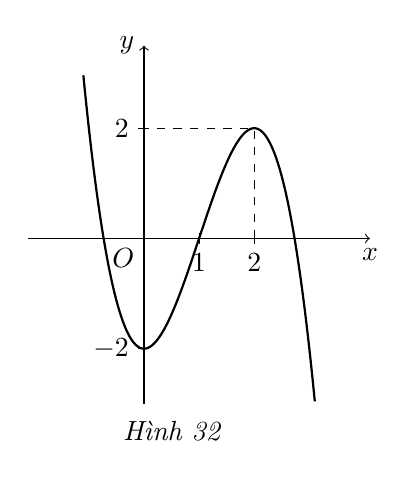
\begin{tikzpicture}[scale=.7]
			
			\def\a{-1}
			\def\b{3}
			\def\c{0}
			\def\d{-2}
			\def\f(#1){\a*((#1)^3)+\b*((#1)^2)+\c*(#1)+\d}
			\def\xmin{-1.1}
			\def\xmax{3.1}
			\def\ymin{-2}
			\def\ymax{2.5}
			\draw[->] (\xmin-1,0)--(\xmax+1,0) node[below] { $x$};
			\draw[->] (0,\ymin-1)--(0,\ymax+1) node[left] { $y$};
			\draw (0,0) node [below left] { $O$};
			\foreach \x in {1,2}\draw (\x,0.1)--(\x,-0.1) node [below] { $\x$};
			\foreach \y in {-2,2}\draw (0.1,\y)--(-0.1,\y) node [left] { $\y$};
			\draw[thick,smooth,samples=200] plot[domain=\xmin:\xmax] (\x,{\f(\x)});
			\draw[dashed] (2,0)|-(0,2);
			\node at (.5,-3.5) {\it Hình 32};
			
		\end{tikzpicture}
	}
	
	\loigiai{
		Dạng đồ thị hàm số đã cho là hàm số bậc ba có hệ số $a<0$ và có hai điểm cực trị $(0;-2)$ và $(2;2)$.
		\begin{itemize}
			\item Xét hàm số $y=-x^3+3x-2$. Ta có $a=-1<0$, $y^\prime=-3x^2+3=0\Leftrightarrow \hoac{&x=-1\\&x=1}$.
			\item Xét hàm số $y=-x^3-2$. Ta có $a=-1<0$, $y^\prime=-3x^2\le 0, \forall x\in \mathbb{R}$.
			\item Xét hàm số $y=-x^3+3x^2-2$. Ta có $a=-1<0$, $y^\prime=-3x^2+6x=0\Leftrightarrow \hoac{&x=0\\&x=2}$.
			\item Xét hàm số $y=x^3-3x-2$. Ta có $a=1>0$.
		\end{itemize}
		Do đó hàm số $y=-x^3+3x^2-2$ thỏa mãn đề bài.
	}
\end{ex}
\begin{ex}%[2D1H1-1]
	\immini[thm]{ 
		Đường cong ở {\it Hình 33} là đồ thị của hàm số nào sau đây?
		\choice[2]
		{$y=\dfrac{x+1}{x-1}$}
		{$y=\dfrac{-x+1}{x+1}$}
		{$y=\dfrac{x-1}{x+1}$}
		{\True $y=\dfrac{-x}{x+1}$}
	}{
		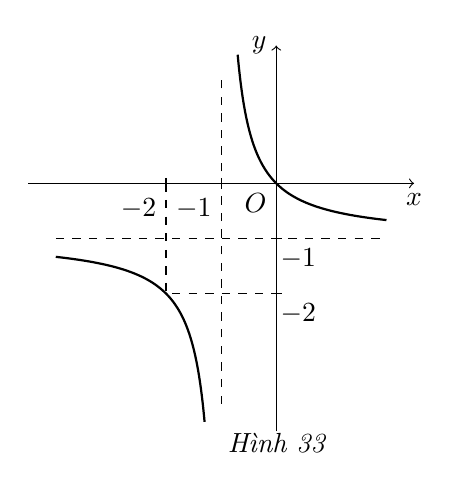
\begin{tikzpicture}[scale=.7]
			
			
			\def\a{-1}
			\def\b{0}
			\def\c{1}
			\def\d{1}
			\def\f(#1){(\a*(#1)+\b)/(\c*(#1)+\d)}
			\def\xmin{-4}
			\def\xmax{2}
			\def\ymin{-4}
			\def\ymax{2}
			\def\m{-\d/\c} %Điểm cận để vẽ đồ thị 
			\def\n{0.3} %hãy thay đổi để biết cụ thể
			\draw[->] (\xmin-.5,0)--(\xmax+.5,0) node[below] { $x$};
			\draw[->] (0,\ymin-.5)--(0,\ymax+.5) node[left] { $y$};
			\draw (0,0) node [below left] { $O$};
			\foreach \x in {-2,-1}\draw (\x,0.1)--(\x,-0.1) node [below left] { $\x$};
			\foreach \y in {-2,-1}\draw (0.1,\y)--(-0.1,\y) node [below right] { $\y$};
			\draw[dashed] (-\d/\c,\ymin)--(-\d/\c,\ymax);
			\draw[dashed] (\xmin,\a/\c)--(\xmax,\a/\c);
			\draw[thick,smooth,samples=200] plot[domain=\xmin:{\m-\n}] (\x,{\f(\x)});
			\draw[thick,smooth,samples=200] plot[domain={\m+\n}:\xmax] (\x,{\f(\x)});
			\draw[dashed] (-2,0)|-(0,-2);
			\node at (0,-4.7) {\it Hình 33};
			
			
		\end{tikzpicture}
	}
	
	\loigiai{
		Dạng đồ thị hàm số đã cho là hàm số $y=\dfrac{ax+b}{cx+d}$ có tiệm cận đứng $x=-1$, tiệm cận ngang $y=-1$ và đi qua điểm $(0;0)$. Suy ra:\\
		$\dfrac{b}{d}=0 \Leftrightarrow b=0$; $-\dfrac{d}{c}=-1\Leftrightarrow d=c$; $\dfrac{a}{c}=-1\Leftrightarrow a=-c$.
		Do đó hàm số $y=\dfrac{-x}{x+1}$ có $-a=c=d=-1, b=0$ thỏa mãn đề bài.
	}
\end{ex}
\Closesolutionfile{ans}
\indapan{6}{ans/ans-2-GK1-De2-LC}

\cauds
\Opensolutionfile{ans}[ans/ans-2-GK1-De2-DS]
\begin{ex}%[2D1V5-1]
Cho hàm số $y=f(x)=x^3+ax^2+bx+c$ có đồ thị như hình vẽ. 
\immini{Xét tính đúng sai của các phát biểu sau
\choiceTF
{Hàm số đống biến trên khoảng $(0;2)$}
{Khoảng cách giữa hai cực trị của hàm số là $2$}
{\True Tổng $a+b+c=-1$}
{\True Hàm số $g(x)=f(f(x))$ đồng biến trên khoảng $(0;1)$}
}{
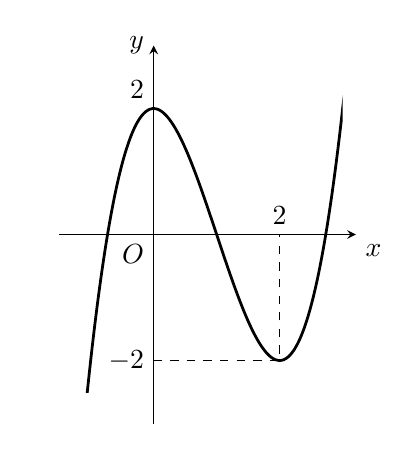
\begin{tikzpicture}[x=1cm,y=1cm,scale=0.8,>=stealth]
	\def\aa{1} \def\bb{-3} \def\cc{0} \def\dd{2}
	\draw[->] (-1.5,0)--(3.21,0)node[below right]{$x$};
	\draw[->] (0,-3)--(0,2)node[above left]{$2$}--(0,3)node[left]{$y$};
	\fill (0,0)node[below left]{$O$};
	\clip (-2,-2.5) rectangle (3,2.8);
	\draw[black,samples=150,smooth,domain=-1.75:3.2,line width=1pt] plot(\x,{\aa*(\x)^3+\bb*(\x)^2+\cc*\x+\dd});
	\draw[dashed](0,-2)node[left]{$-2$}--(2,-2)--(2,0)node[above]{$2$};
\end{tikzpicture}
}
\loigiai{
\begin{itemchoice}
	\itemch Sai. Dễ thấy hàm số $f(x)$ nghich biến trên $(0;2)$
	\itemch Sai. Hàm số có cực đại là $y_{\text{CĐ}}=2$ và có cực tiểu là $y_{\text{CT}}=-2$, do đó khoảng cách giữa hai cực trị là $|y_{\text{CĐ}}-y_{\text{CT}}|=4$.
	\itemch Đúng. Đồ thị hàm số có hai điểm cực trị là $A(0;2)$ và $B(2;-2)$; khi đó tọa độ trung điểm $AB$ là $I(1;0)$ là tâm đối xứng của đồ thị, cũng là điểm uốn của đồ thị nên $f(1)=0\Leftrightarrow a+b+c=-1$. 
	\itemch Đúng. Ta có $g'(x)=f'(x)\cdot f'(f(x))$.\\
	Dựa vào đồ thị hàm số ta có $f(x)$ nghịch biến trên $(0;2)$ nên $f'(x)\leq 0, \forall x\in (0;2)$.\\
	Khi $x\in (0;1)$ ta có $$\heva{&f'(x)\leq 0\\&f(x)\in (0;2)}\Rightarrow \heva{&f'(x)\leq 0\\&f'(f(x))\leq 0}\Rightarrow g'(x)=f'(x)\cdot f'(f(x))\geq 0, \forall x\in (0;1).$$
	Vậy hàm số $g(x)$ đồng biến trên $(0;1)$.
\end{itemchoice}
}
\end{ex}
\begin{ex}%[2D1H5-1]
Cho hàm số $y=f(x)=\dfrac{ax+b}{cx+d}$ có bảng biến thiên như hình vẽ.
\immini{\choiceTF
{\True Đồ thị hàm số nhận đường thẳng $x=1$ làm tiệm cận đứng}
{ Hàm số đã cho nghịch biến trên $\mathbb{R}\setminus\{1\}$}
{\True Tâm đối xứng của đồ thị hàm số là $I(1;2)$}
{Có $2024$ số nguyên $m$ trên $[-2024;2024]$ để phương trình $\left|\dfrac{ax+b}{cx+d}\right|=m$ có $2$ nghiệm phân biệt}
}
{
\begin{tikzpicture}[>=stealth]
		\tkzTabInit[nocadre=false,lgt=1,espcl=2,deltacl=0.5]{$x$/.7 ,$y'$/.7,$y$/2}
		{$-\infty$ , $1$ , $+\infty$}
		\tkzTabLine{ , - , d , - , }
		\tkzTabVar{+/$2$ , -D+/$-\infty$/$+\infty$ , -/$2$}
	\end{tikzpicture}
}
\begin{itemchoice}
	\itemch Đúng. Đồ thị hàm số nhận đường thẳng $x=1$ làm tiệm cận đứng.
	\itemch Sai. Hàm số nghịch biến trên các khoảng $(-\infty;1)$ và $(1;+\infty)$. Không nghịch biến trên $\mathbb{R}\setminus \{1\}$ vì $f(5)>2>f(0)$.
	\itemch Đúng. Đồ thị hàm số nhận đường thẳng $y=2$ làm tiệm cận ngang, do đó tâm đối xứng của đồ thị hàm số là $I(1;2)$.
	\itemch Sai. Từ bảng biến thiên của hàm số $f(x)$ ta có bảng biến thiên của hàm số $|f(x)|$ như sau (ở đây $x_0=-\dfrac{b}{a}$).
\begin{center}
\begin{tikzpicture}[>=stealth]
		\tkzTabInit[nocadre=false,lgt=1,espcl=2,deltacl=0.5]{$x$/.7 ,$y'$/.7,$y$/2}
		{$-\infty$ , $x_0$ , $1$ , $+\infty$}
		\tkzTabLine{ , - , d , + , d , - , }
		\tkzTabVar{+/$2$ , -/$0$ , +D+/$+\infty$/$+\infty$ , -/$2$}
\end{tikzpicture}\end{center}
Dựa vào bảng biến thiên ta thấy phương trình $\left|\dfrac{ax+b}{cx+d}\right|=m$ có $2$ nghiệm phân biệt khi và chỉ khi $2\neq m >0$, do đó có $2023$ giá trị nguyên của tham số $m$ thỏa yêu cầu.
\end{itemchoice}
\end{ex}
\begin{ex}%[2D1V5-1]
\immini{Cho hàm số $y=\dfrac{ax^2+bx+c}{mx-1}$ có đồ thị như hình vẽ. Xét tính đúng sai của các phát biểu sau
\choiceTF
{\True Đồ thị hàm số nhận đường thẳng $x=1$ làm tiệm cận đứng}
{\True Đồ thị hàm số nhận điểm $I(1;1)$ làm tâm đối xứng}
{Giá trị của $a+b+c+m$ bằng $1$}
{\True Đường thẳng đi qua hai điểm cực trị của đồ thị hàm số là $y=2x+1$}
		}{
			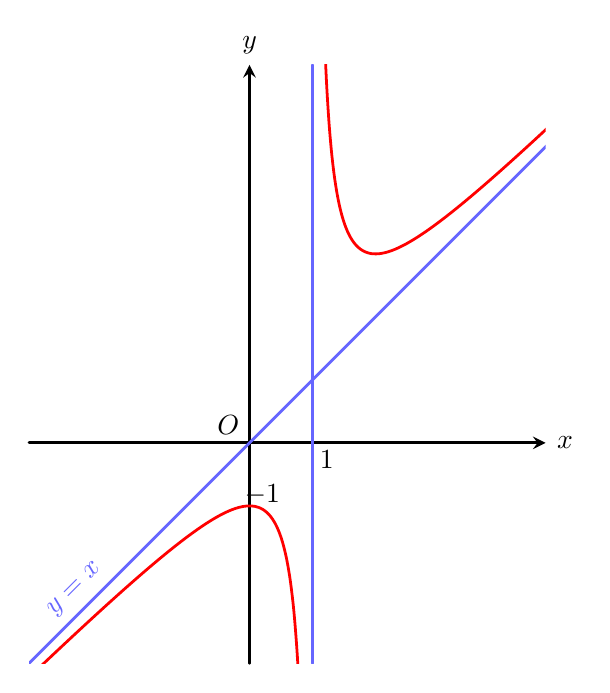
\begin{tikzpicture}[>=stealth,scale=0.8, line join=round, line cap=round, line width=1pt]
				\tikzset{declare function={xmin=-3.5;xmax=4.7;ymin=-3.5;ymax=6;},
					smooth,samples=450}
				\draw[->] (xmin,0)--(xmax,0) node[shift={(0:7pt)}]{$ x $};
				\draw[->] (0,ymin)--(0,ymax) node[shift={(90:7pt)}]{$ y $};
				\fill (0,0) node[shift={(140:10pt)}]{$ O $};
				\clip (xmin,ymin) rectangle (xmax,ymax);
				\draw(0,-1)node[shift={(40:6pt)}]{$-1$};
				\draw(1,0)node[shift={(-50:8pt)}]{$1$};
				\def\f(#1){((#1)^2-(#1)+1)/((#1)-1)}
				\def\a{-1}
				\def\b{0}
				\def\c{0.5}
				\def\d{1.5}	
				\def\e{2}
				\def\g{3}	
				\pgfmathsetmacro\fa{\f(\a)}
				\pgfmathsetmacro\fb{\f(\b)}
				\pgfmathsetmacro\fc{\f(\c)}
				\pgfmathsetmacro\fd{\f(\d)}	
				\pgfmathsetmacro\fe{\f(\e)}
				\pgfmathsetmacro\fg{\f(\g)}	
				\draw[red,samples=100] plot[domain=-5.3:0.9] (\x,{\f(\x)});	
				\draw[red,samples=100] plot[domain=1.05:5.2] (\x,{\f(\x)});
				\draw[blue!60] (1,ymin)--(1,ymax);
				\draw[blue!60] (xmin,ymin)--(6,ymax)node [pos=0.1,sloped, above]{$y=x$};
			\end{tikzpicture}
		}
	\loigiai{
	\begin{itemchoice}
		\itemch Đúng. Dựa vào đồ thị hàm số ta thấy đường thẳng $x=1$ là đường tiệm cận đứng của đồ thị hàm số.
		\itemch Đúng. Dựa vào đồ thị hàm số ta thấy tiệm cận xiên của đồ thị hàm số là $y=x$, do đó tâm đối xứng của đồ thị hàm số là giao điểm của tiệm cận đứng và tiệm cận xiên nên tọa độ tâm đối xứng là $I(1;1)$.
		\itemch Sai. Dựa vào đồ thị hàm số ta có $x=0$ thì $y=-c=-1\Leftrightarrow c=1$.\\
		Đường tiệm cận đứng của đồ thị hàm số là $x=1$ nên $m=1$.\\
		Ta có $y=\dfrac{ax^2+bx+1}{x-1}=a(x+1)+b+\dfrac{a+b+1}{x-1}$ có đường tiệm cận xiên là $y=x$ nên $\heva{&a=1\\&a+b=0}\Leftrightarrow \heva{&a=1\\&b=-1.}$\\
		Vậy $T=a+b+c+m=2$.
		\itemch Đúng. Như vậy ta có hàm số đã cho được viết lại là $y=\dfrac{x^2-x+1}{x-1}$ nên đường thẳng đi qua hai điểm cực trị của đồ thị hàm số là $y=2x-1$.
\end{itemchoice}					}
\end{ex}
\begin{ex}%[2D1H5-1]
Một chất điểm chuyển động theo phương trình li độ $x(t)=-t^3+18t^2+t+3$, trong đó $t$ tính bằng giây và $x$ tính bằng mét. Xét tính đúng sai của các phát biểu sau
\choiceTF
{\True Li độ của chất điểm ở thời điểm $t=4$ giây là $231$ mét}
{\True Vận tốc của chất điểm tại thời điểm $t=5$ giây là $106\, \mathrm{(m/s)}$}
{Gia tốc của chất điểm tại thời điểm $t=10$ giây là $24\, \mathrm{(m/s^2)}$}
{Khi vận tốc của chất điểm đạt giá trị lớn nhất thì li độ của chất điểm là $231\, (m)$}
	\loigiai{
	\begin{itemchoice}
		\itemch Đúng. Li độ của chất điểm ở thời điểm $t=4$ giây là $x(4)=231\, (m)$.
		
		\itemch Đúng. Ta có $v(t)=x'(t)=-3t^2+36t+1$, suy ra vận tốc của chất điểm ở thời điểm $t=5$ giây là $v(5)=106\, \mathrm{(m/s)}$
		
		\itemch Sai. Ta có $a(t)=v'(t)=x''(t)=-6t+36$. Do đó gia tốc tại thời điểm $t=10$ giây là $a(10)=-24\, \mathrm{(m/s^2)}$
		
		\itemch Sai. Ta có $v(t)=x'(t)=-3t^2+36t+1=109-3(t-6)^2\leq 109$. Do đó giá trị lớn nhất của vận tốc là $109\,\mathrm{m/s}$ đạt khi $t=6$ giây.\\
		Lúc đó li độ của chất điểm là $x(6)=441\, \mathrm{(m)}$.
		
\end{itemchoice}					}
\end{ex}

\Closesolutionfile{ans}
\indapan{3}{ans/ans-2-GK1-De2-DS}

\Opensolutionfile{ans}[ans/ans-2-GK1-De2-KQ]
\caukq
	\begin{ex}%[2D1V5-1]
	\immini{
		Cho hàm số bậc ba $y=f(x)=ax^3+bx^2+cx+d$, với $a\neq 0$ có đồ thị như Hình $3$. Hãy tính giá trị của $a+b+c-d$.
	}{
		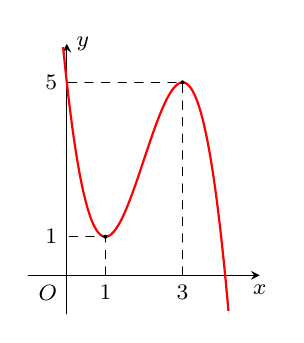
\begin{tikzpicture}[scale=0.7, font=\footnotesize, line join=round, line cap=round, >=stealth, xscale=0.7, yscale=0.7]
			\def\a{-1} \def\b{6} \def\c{-9} \def\d{5} % Hệ số
			\def\xt{-1} \def\xp{5} \def\yt{6} \def\yd{-1} % x_trái, x_phải, y_trên, y_dưới (giới hạn)
			\draw[->] (\xt,0)--(\xp,0) node [below]{$x$};
			\draw[->] (0,\yd)--(0,\yt) node [right]{$y$};
			\node at (0,0) [below left]{$O$};
			\clip (\xt+0.1,\yd+0.1) rectangle (\xp-0.1,\yt-0.1);
			\draw[thick,smooth,samples=300,red] plot(\x,{\a*(\x)^3+\b*(\x)^2+\c*(\x)+\d});
			\draw[dashed] (1,0)node [below]{$1$}--(1,1)--(0,1)node [left]{$1$} (3,0)node [below]{$3$}--(3,5)--(0,5)node [left]{$5$};
			\fill (1,1) circle (1.5pt); \fill (3,5) circle (1.5pt);
		\end{tikzpicture}
	}
\shortans{$-9$}
	\loigiai{
		Ta có $f'(x)=3ax^2+2bx+c$.\\
		Từ hình vẽ ta thấy
		$$\heva{& f(1)=1\\& f(3)=5\\& f'(1)=0\\& f'(3)=0} \Leftrightarrow \heva{& a+b+c+d=1\\& 27a+9b+3c+d=5\\& 3a+2b+c=0\\& 27a+6b+c=0} \Leftrightarrow \heva{& a=-1\\& b=6\\& c=-9\\& d=5.}$$
		Vậy $a+b+c-d=-9$.
	}
\end{ex}
\begin{ex}%[2D1B2-1]
	Tìm giá trị cực đại của hàm số $y=x^{3}-6 x^{2}+9 x+30$.
	\shortans{$34$}
	\loigiai{
		Tập xác định của hàm số là $\mathbb{R}$.
		
		Ta có: $y^{\prime}=3 x^{2}-12 x+9 ; y^{\prime}=0 \Leftrightarrow x=1$ hoặc $x=3$.
		
		Lập bảng biến thiên của hàm số:
		
		\begin{center}
			
\begin{tikzpicture}
				\tkzTabInit[nocadre,lgt=1.2,espcl=2.5,deltacl=0.6]
				{$x$ /0.6,$y'$ /0.6,$y$ /1.5}
				{$-\infty$,$1$,$3$,$+\infty$}
				\tkzTabLine{,+,$0$,-,0,+}
				\tkzTabVar{-/$-\infty$,+/$34$,-/$30$,+/$+\infty$}
			\end{tikzpicture}
		\end{center}
		Từ bảng biến thiên, ta có:\\
		Hàm số đạt cực đại tại $x=1$ và $y_{\text{CĐ}}=y(1)=34$.
	}
\end{ex}

\begin{ex}%[2D1H3-6]
	Hộp sữa $1$ lít được thiết kế dạng hình hộp chữ nhật với đáy là hình vuông cạnh $x$ cm. Tìm $x$ để diện tích toàn phần của hộp nhỏ nhất.
	\shortans{$10$}
	\loigiai{
		Thể tích hộp sữa là $1\ \mathrm{l}=1\ \mathrm{dm}^3=1000\ \mathrm{cm}^3$ khi đó chiều cao của hộp sữa là $\dfrac{1000}{x^2}$ (cm).\\
		Đặt diện tích toàn phần của hộp sữa là $y=2x^2+4x\cdot \dfrac{1000}{x^2}=\dfrac{2x^3+4000}{x}$ (cm)$^2$.\\
		Xét $y'=\dfrac{4x^3-4000}{x^2}=0\Leftrightarrow x=10$ (cm).\\
		Ta có bảng biến thiên như sau
		\begin{center}
			
\begin{tikzpicture}[font=\normalsize,t style/.style={style=solid}]
				%dòng khai báo
				\tkzTabInit[lgt=1,espcl=2.65,deltacl=0.6]
				{$x$ /0.75, $y'$/0.75, $y$/2}
				{$ 0$,$ 10 $,$ +\infty$}
				%dòng xét dấu
				\tkzTabLine{  , -,0 , +,  }  % z, t, d;
				%dòng biến thiên
				\tkzTabVar{+/$+\infty$,-/$600$,+/$+\infty$} %+ hoac-
			\end{tikzpicture}
		\end{center}
		Vậy theo bảng biến thiên ta thấy $x=10$ (cm) thì diện tích toàn phần của hộp sữa sẽ nhỏ nhất là $600\ {\rm cm^2}$. }
\end{ex}
\begin{ex}%[2D1H3-6]
	Khi máu di chuyển từ tim qua các động mạch chính rồi đến các mao mạch và quay trở lại qua các tĩnh mạch, huyết áp tâm thu (tức là áp lực của máu lên động mạch khi tim co bóp) liên tục giảm xuống. Giả sử một người có huyết áp tâm thu $P$ (tính bằng mmHg) được cho bởi hàm số
	$$
	P(t)=\dfrac{25 t^2+125}{t^2+1}, 0 \leq t \leq 10,
	$$
	trong đó thời gian $t$ được tính bằng giây. Tính tốc độ thay đổi của huyết áp sau $5$ giây kể từ khi máu rời tim.
		\shortans{$-0{,}74$}
	\loigiai{
		Ta có tốc độ thay đổi của huyết áp là $P'(t)=\dfrac{-100t}{(t^2+1)^2}$.\\
		Do đó tốc độ thay đổi huyết áp sau $5$ s là $P'(5)=-\dfrac{125}{169}\approx -0{,}74$.
	}
\end{ex}

\begin{ex}%[2D1H3-6]
	Một nhà sản xuất cần làm những hộp đựng hình trụ có thể tích $ 1 $ lít. Tìm các kích thước của hộp đựng để chi phi vật liệu dùng để sản xuất là nhỏ nhất (kết quả được tính theo centimét và làm tròn đến chứ số thập phân thứ hai).
		\shortans{$10{,}84$}
	\loigiai{
		Đổi $1 \text{ lít} =1000 \text{ cm}^3$.
		\\
		Gọi $r( cm )$ là bán kính đáy của hình trụ, $h( cm )$ là chiều cao của hình trụ.
		\\
		Diện tích toàn phần của hinh trụ là $S=2 \pi r^2+2 \pi r h$.
		\\
		Do thể tích của hình trụ là $1000 \text{ cm}^3$ nên ta có: $1000=V=\pi r^2 h$, hay $h=\dfrac{1000}{\pi r^2}$.
		\\
		Do đó, diện tích toàn phần của hình trụ là $S=2 \pi r^2+\dfrac{2000}{r},\, r>0$.
		\\
		Ta cần tìm $r$ sao cho $S$ đạt giá trị nhỏ nhất. Ta có
		\begin{align*}
			&S'=4 \pi r-\dfrac{2000}{r^2}=\dfrac{4 \pi r^3-2000}{r^2};
			\\
			&S'=0 \Leftrightarrow \pi r^3=500 \Leftrightarrow r=\sqrt[3]{\dfrac{500}{\pi}}
		\end{align*}
		Bảng biến thiên
		\begin{center}
			
\begin{tikzpicture}[font=\footnotesize,thick,>=stealth]
				\tikzset{double style/.append style={double distance=1.5pt}}\tkzTabInit[nocadre=false,lgt=1.2,espcl=3.5,deltacl=0.6,lw=.75pt,color,colorL=green!50,colorV=green!50]
				{$r$ /1.2, $S'(r)$ /1, $S(r)$ /2.5}
				{$0$,$\sqrt[3]{\dfrac{500}{\pi}}$,$+\infty$}
				\tkzTabLine{ ,-,$0$,+, }
				\tkzTabVar{+/$+\infty$,-/$S\left( \sqrt[3]{\dfrac{500}{\pi}} \right)$,+/$+\infty$}
			\end{tikzpicture}
		\end{center}
		Khi đó
		$$
		h=\dfrac{1000}{\pi r^2}=\dfrac{1000}{\pi \sqrt[3]{\frac{250000}{\pi^2}}}=\dfrac{100}{\sqrt[3]{250 \pi}}.
		$$
		Vậy cần sản xuất các hộp đựng hình trụ có bán kinh đáy $r=\sqrt[3]{\dfrac{500}{\pi}} \approx 5,42 \text{ (cm)}$ và chiều cao $h=\dfrac{100}{\sqrt[3]{250 \pi}} \approx 10,84\text{ (cm)}$.
	}
\end{ex}
\begin{ex}%[2D1H1-1]
	Một đường dây điện được nối từ một nhà máy điện ở $A$ đến một hòn đảo ở $C$ như Hình 1.40. Khoảng cách từ $C$ đến $B$ là $4$ $\mathrm{km}$. Bờ biển chạy thẳng từ $A$ đến $B$ với khoảng cách là $10$ $\mathrm{km}$. Tổng chi phí lắp đặt cho $1$ $\mathrm{km}$ dây điện trên biển là $50$ triệu đồng, còn trên đất liền là $30$ triệu đồng. Điểm $M$ trên đoạn $AB$ khoảng bao nhiêu km (điểm nối dây từ đất liền ra đảo) để tổng chi phí lắp đặt là nhỏ nhất.
\shortans{$3$}
	\begin{center}
		\begin{tikzpicture}[scale=1, font=\footnotesize, line join=round, line cap=round, >=stealth]
			%%%%%%%%%%%%%%%%%%%%%%%%%%%%%%%%%
			\fill (10,0) circle(1pt) node[right]{$A$};
			\fill (0,0) circle(1pt) node[left]{$B$};
			\fill (3,0) circle(1pt) node[below]{$M$};
			\fill (0,4) circle(1pt) node[above]{$C$};
			\fill (0,2) circle(0pt) node[left]{$4 \mathrm{km}$};
			%%%%%%%%%%%%%%%%%%%%%%%%%%%%%%%%%
			\draw (0, 0) -- (0, 4) -- (3, 0) -- (10, 0) -- (0, 0); 
			%%%%%%%%%%%%%%%%%%%%%%%%%%%%%%%%%
		\end{tikzpicture} \\
		Hình 1.40
	\end{center}
	\loigiai{
		Đặt $MB=x(\mathrm{km}, 0\le x\le 10)$ $\Rightarrow AM=10-x$ (km), $MC=\sqrt{MB^2+CB^2}=\sqrt{x^2+16}(\mathrm{km})$.\\
		Khi đó, chi phí nối điện từ $A$ đến $C$ là $f(x)=30(10-x)+50\sqrt{x^2+16}$ (triệu đồng). \\ 
		Ta có $f'(x)=-30+\dfrac{50x}{\sqrt{x^2+16}}$. \\ 
		$f'(x)=0\Leftrightarrow \dfrac{x}{\sqrt{x^2+16}}=\dfrac{3}{5}\Leftrightarrow 25x^2=9x^2+144\Leftrightarrow x=3$ (do $0 \le x \le 10$).\\
		Ta có $f(0)=500$, $f(3)=460$, $f(10)=100 \sqrt{29}$ nên chi phí nhỏ nhất là $460$ triệu đồng khi $x=3$.\\
		Vậy $M$ cách $B$ một khoảng $3$ $\mathrm{km}$ trên đoạn $AB$ (điểm nối dây từ đất liền ra đảo) thì tổng chi phí lắp đặt là nhỏ nhất.
	}
\end{ex}
%\begin{ex}%[0D3N1-3]
%	Cho hàm số $y=f(x)=\dfrac{x^2+2}{x-1}$. Giá trị của hàm số tại $x=5$ bằng bao nhiêu?
%	\shortans{$6{,}75$}
%	\loigiai{
%		Ta có $f\left(5\right)=\dfrac{5^2+2}{4}=\dfrac{27}{4}=6{,}75$.
%	}
%\end{ex}

\Closesolutionfile{ans}
\indapan{6}{ans/ans-2-GK1-De2-KQ}

